\section{Measurement Strategy}
\label{sec:measurement-strategy}

The Phase-I \(R_{e/\mu}\) measurement is a stopped-pion counting experiment.
A positive pion is brought to rest in an active target and decays either
directly through \(\pi^{+}\to e^{+}\nu_e(\gamma)\), or through the dominant
sequential chain \(\pi^{+}\to\mu^{+}\nu_\mu\) followed by
\(\mu^{+}\to e^{+}\nu_e\bar{\nu}_\mu\). The calorimeter measures the outgoing
positron energy, while the active target (ATAR) records the five-dimensional space-time-energy
patterns of the charged particles. In this way the ATAR tracks the pion stop, the possible
intermediate muon stop, and the early space-time pattern of outgoing positrons.

\subsection{Energy and Timing Separation}
\label{subsec:measurement-energy-timing}

The basic separation is set by two-body pion decay kinematics and by the
large difference between the pion and muon lifetimes. At rest, the pion
lifetime is approximately \(\withunit{26}{\nano\second}\), while the muon
lifetime is approximately \(\withunit{2.2}{\micro\second}\). The direct decay
\(\pi^{+}\to e^{+}\nu_e\) produces a monoenergetic positron with energy near
\(\withunit{69.8}{\mega\electronvolt}\), while positrons from ordinary muon
decay follow the continuous Michel spectrum up to an endpoint near
\(\withunit{52.8}{\mega\electronvolt}\) \cite{PDG2024}. In an ideal detector,
a high-energy positron therefore tags the direct pion decay, while a
lower-energy positron tags the \(\pi\to\mu\to e\) chain. Illustrative energy
spectra for the two channels are shown in
\figref{fig:measurement-ideal-energy-spectrum}, while the corresponding timing
separation is illustrated in
\figref{fig:measurement-timing-spectrum}.

The analysis separates reconstructed positrons into high- and low-energy
regions using a threshold
\begin{equation}
  E_{\mathrm{cut}} \simeq \withunit{56}{\mega\electronvolt}.
\end{equation}
The high-energy region is dominated by \(\pi\to e\nu\), and the low-energy
region is dominated by \(\pi\to\mu\to e\). The time spectra in the two energy regions are then fit using the prompt
\(\pi\to e\nu\) shape, the delayed \(\pi\to\mu\to e\) shape, and background
components from pileup, pion decays in flight, muon decays in flight, and old
muons left from earlier pion stops \cite{pioneer_proposal_2022,pioneer_rare_2022}.

\subsection{Corrections}
\label{subsec:measurement-corrections}

The raw high-to-low count ratio is not by itself the final branching-ratio
measurement. It must be multiplied by correction factors that account for
detector response, event classification, and analysis selection effects. In
schematic form,
\begin{equation}
  R_{e/\mu}
  =
  \frac{N_H}{N_L}
  \times
  \left(\text{correction factors}\right).
  \label{eq:remu-schematic-corrections}
\end{equation}

Two correction classes are central to the Phase-I strategy. The first is the
calorimeter tail correction: finite detector resolution, shower leakage,
photonuclear interactions, radiative decays, and geometric acceptance move
some true \(\pi\to e\nu\) events below \(E_{\mathrm{cut}}\), where they sit
under the much larger Michel spectrum. Even in an otherwise idealized detector,
finite energy resolution broadens the reconstructed positron spectra and
produces overlap between the high- and low-energy regions, as illustrated in
\figref{fig:measurement-positron-tail-correction}. This tail was a leading
systematic uncertainty in PIENU, and PIONEER reduces it with a deep,
high-resolution, large-solid-angle calorimeter combined with active-target
event classification \cite{pioneer_proposal_2022,pioneer_rare_2022}. The
second class is the relative efficiency and acceptance correction. Direct
\(\pi\to e\nu\) events and sequential \(\pi\to\mu\to e\) events are not
triggered, reconstructed, classified, or accepted with exactly the same
probability.

\begin{figure}[htbp]
  \centering
  \begin{subfigure}[t]{0.49\textwidth}
    \centering
    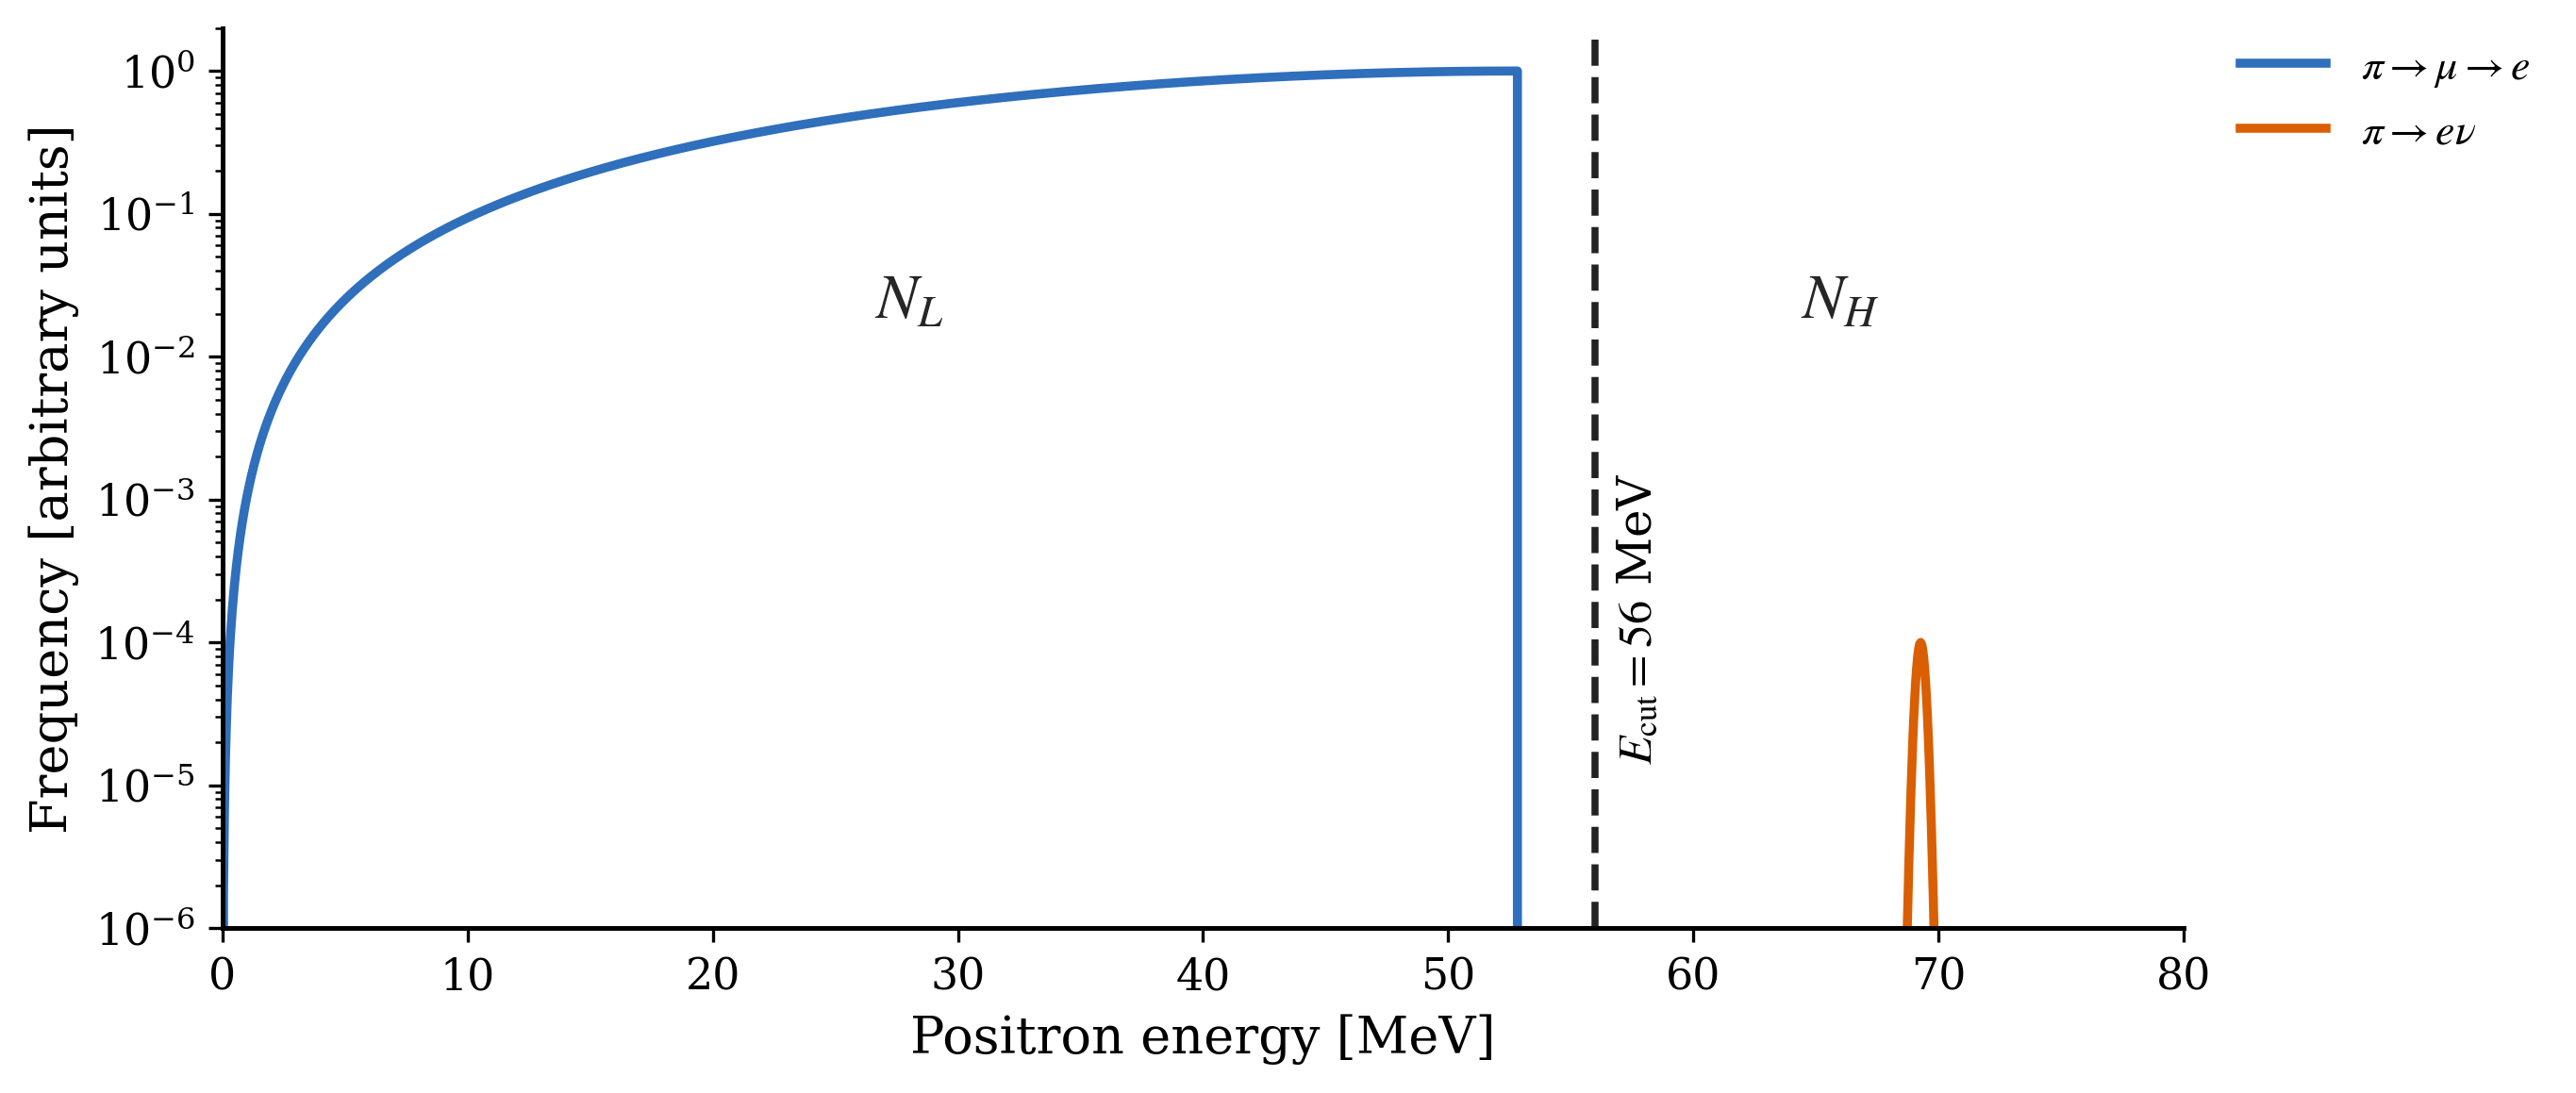
\includegraphics[width=\textwidth]{../resources/figures/chapters/01_introduction/ideal_positron_energy_spectra}
    \caption{Ideal energy separation.}
    \label{fig:measurement-ideal-energy-spectrum}
  \end{subfigure}
  \hfill
  \begin{subfigure}[t]{0.42\textwidth}
    \centering
    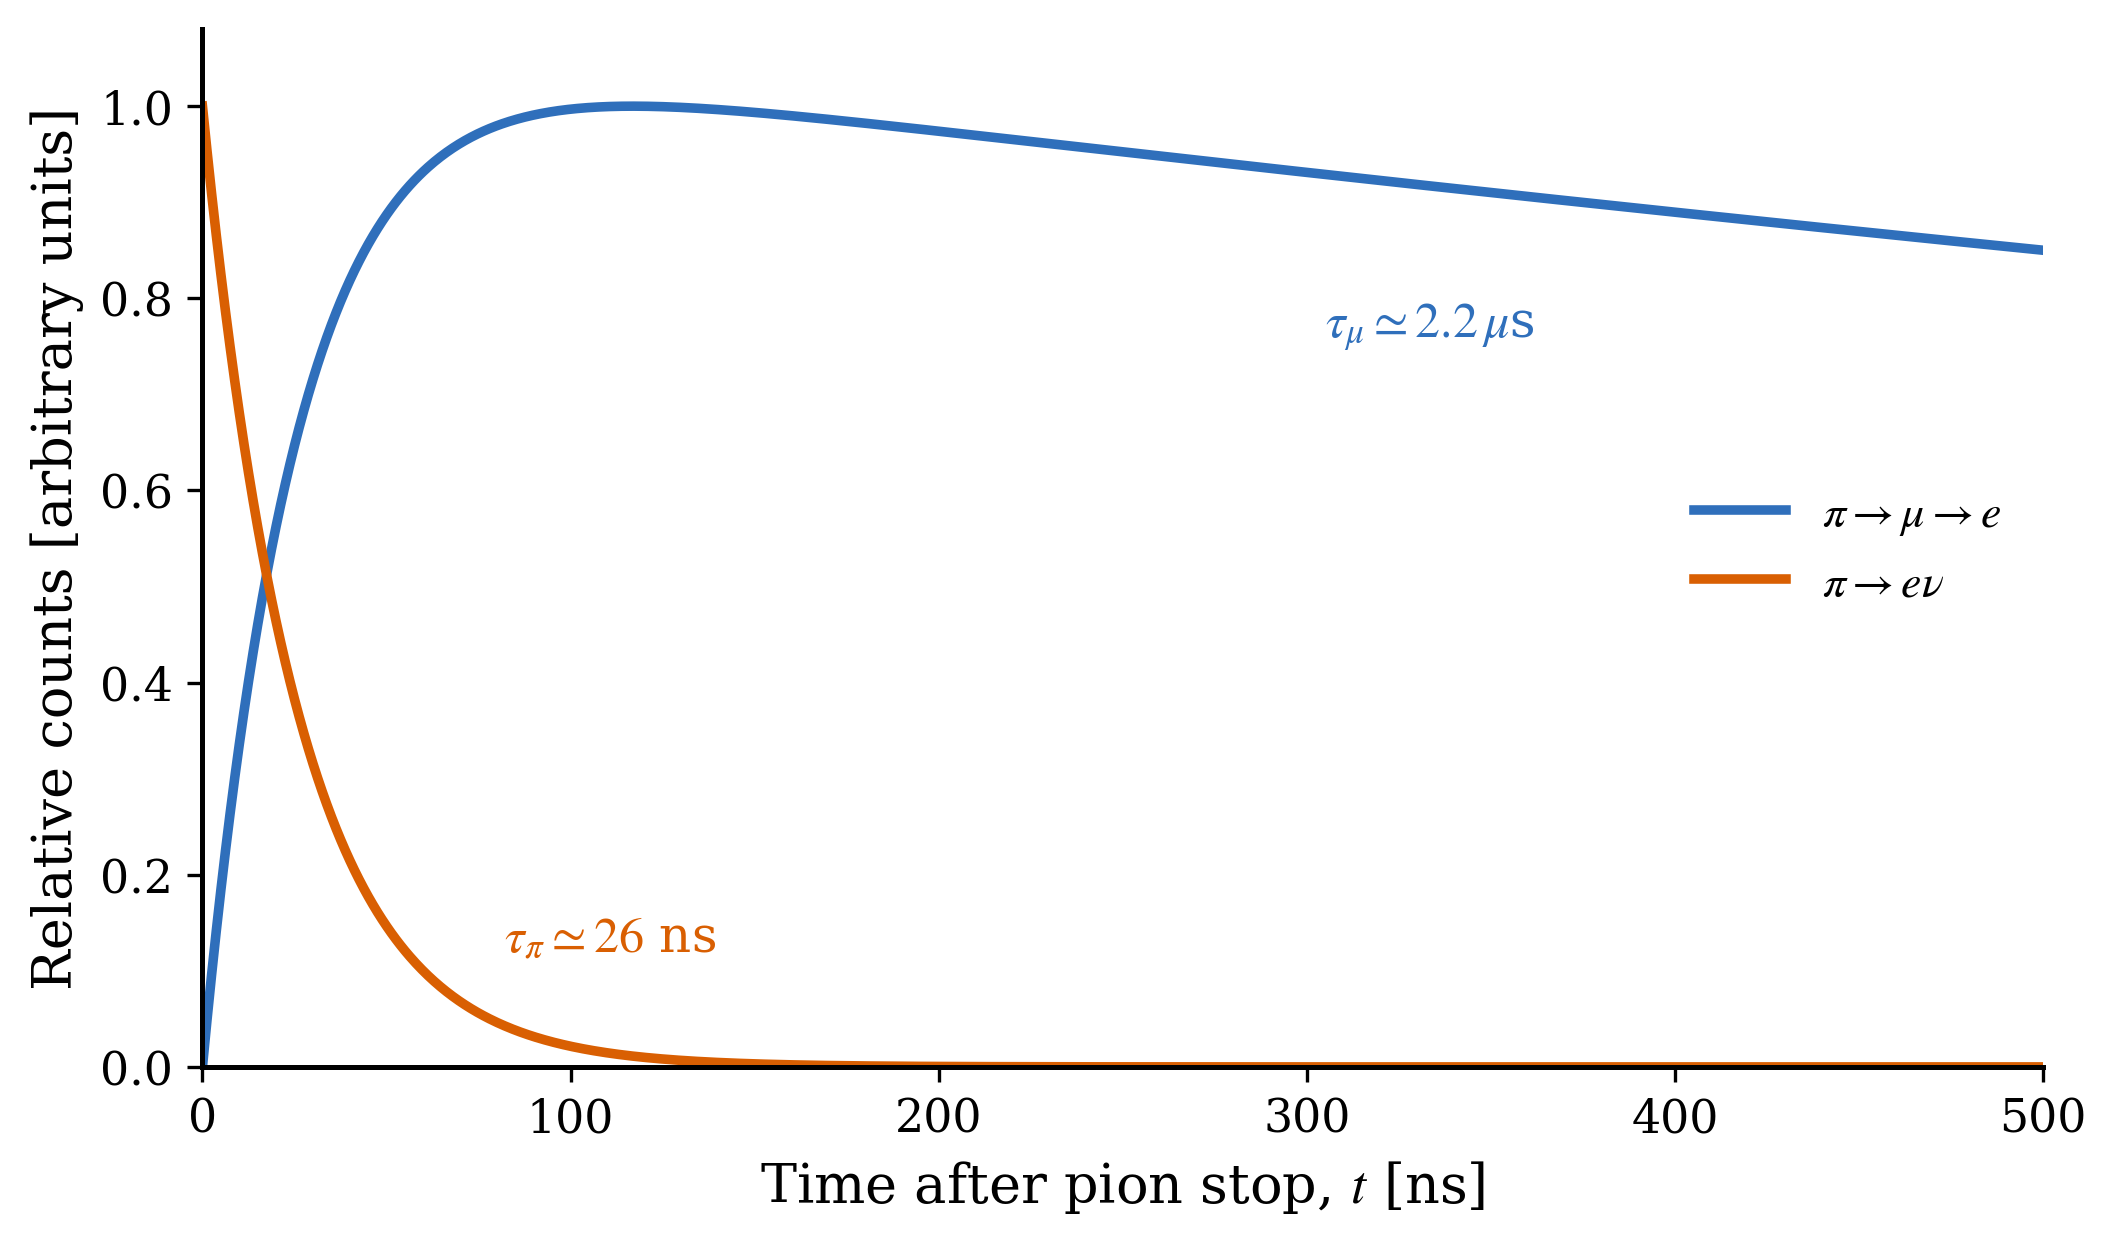
\includegraphics[width=\textwidth]{../resources/figures/chapters/01_introduction/timing_separation_prompt_view}
    \caption{Prompt and delayed timing.}
    \label{fig:measurement-timing-spectrum}
  \end{subfigure}

  \vspace{0.6em}

  \begin{subfigure}[t]{0.54\textwidth}
    \centering
    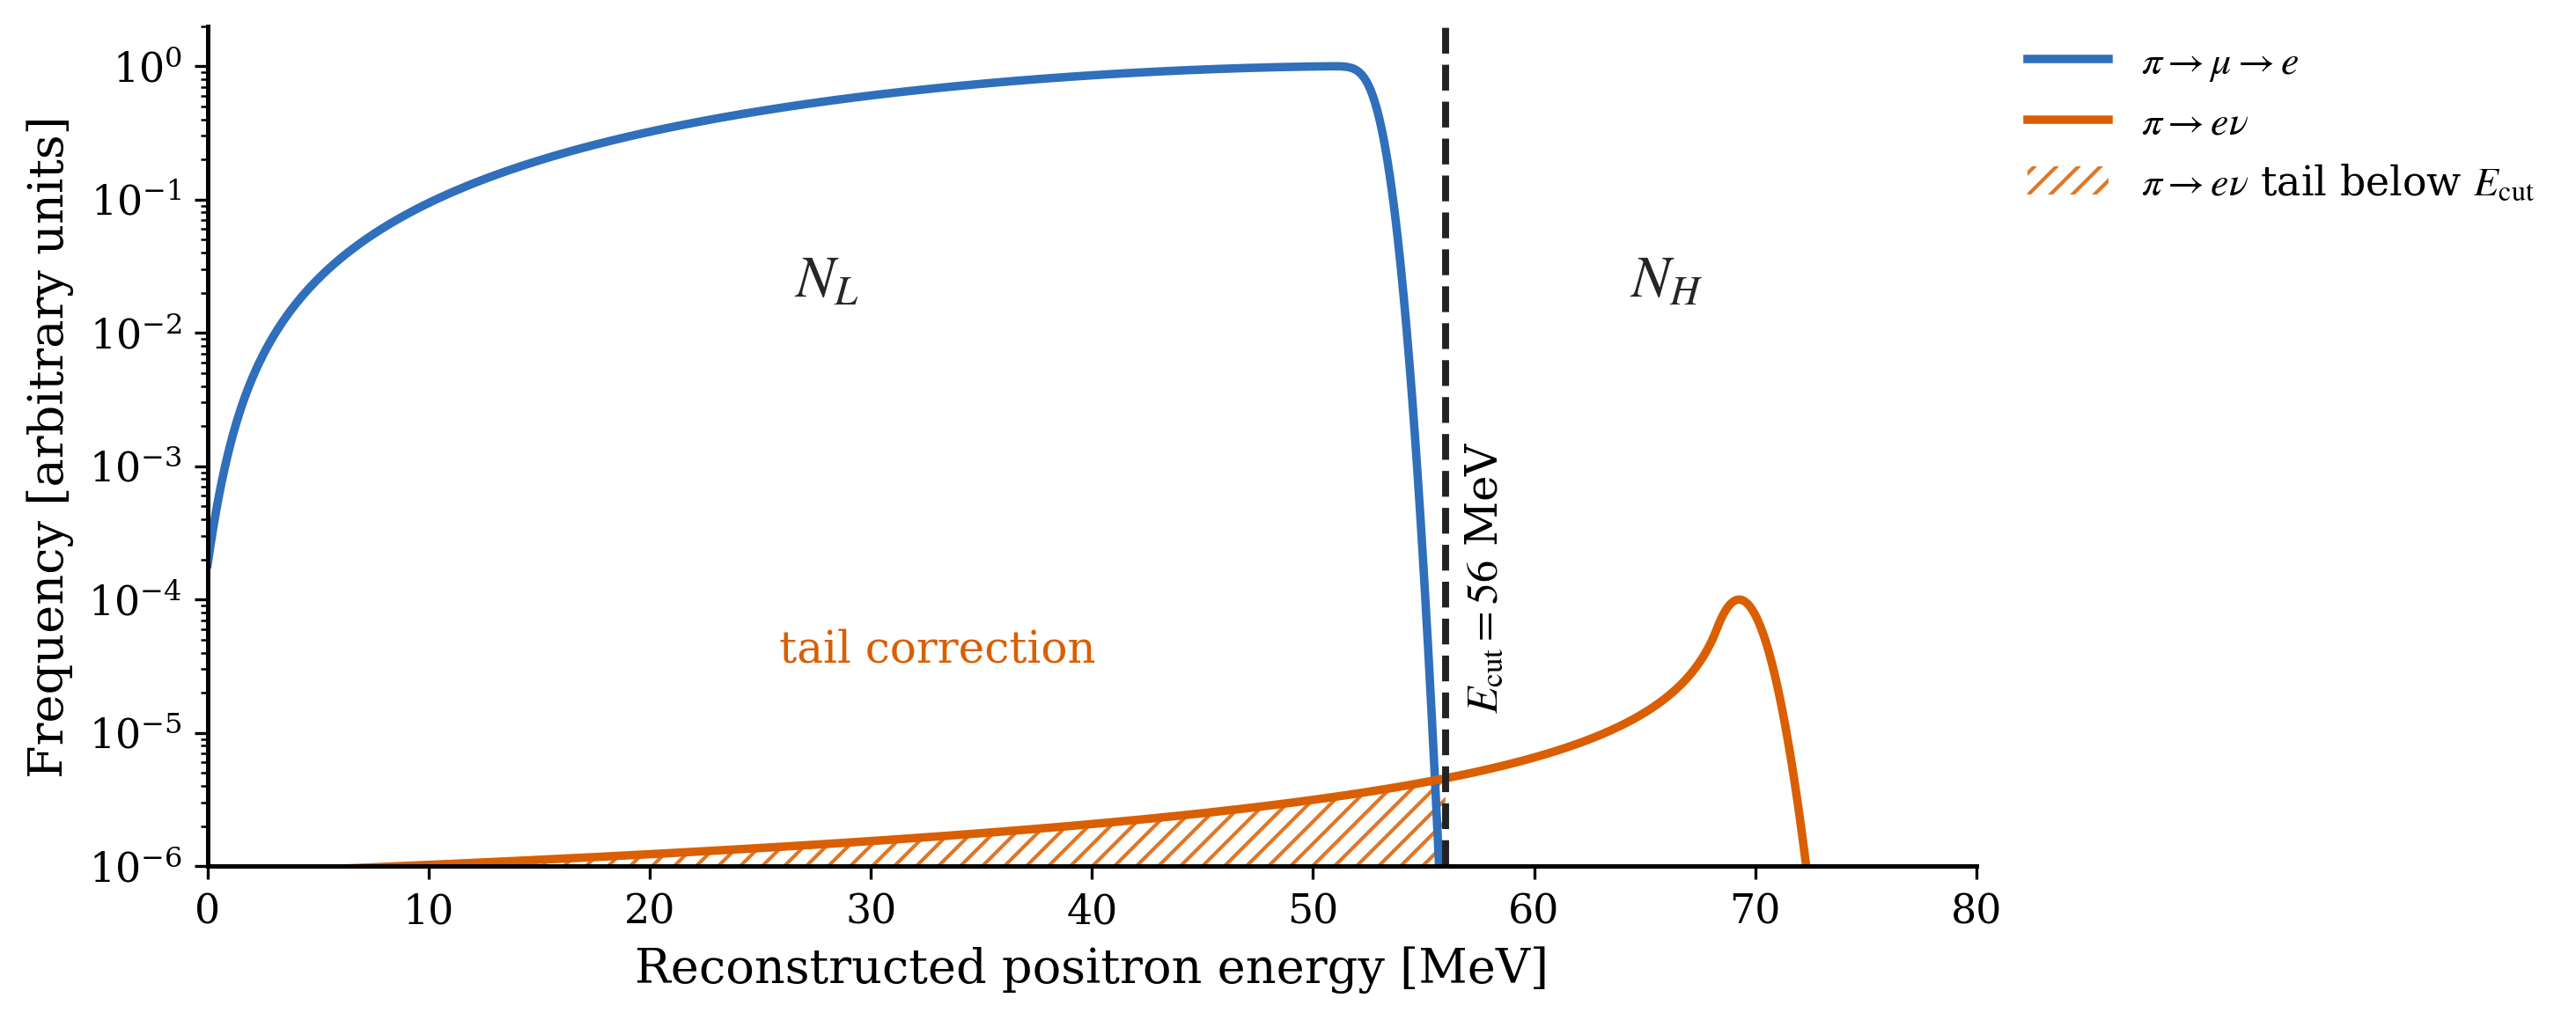
\includegraphics[width=\textwidth]{../resources/figures/chapters/01_introduction/positron_tail_correction}
    \caption{Low-energy signal tail.}
    \label{fig:measurement-positron-tail-correction}
  \end{subfigure}

  \caption{Pedagogical spectra used in the Phase-I \(R_{e/\mu}\) strategy.
  Energy and timing separate the direct and sequential decay channels, while
  finite calorimeter response moves some \(\pi\to e\nu\) events below
  \(E_{\mathrm{cut}}\).}
  \label{fig:measurement-strategy-spectra}
\end{figure}

These corrections also depend on the reconstructed positron
direction. The detector geometry is approximately symmetric under rotations
about the beam axis, but the response is not fully uniform because of the
forward beam entrance region, upstream material, target geometry, calorimeter
containment, reconstruction thresholds, and the directional segmentation of
the active target planes. In particular, the alternating vertical and
horizontal strip geometry of the active target produces direction-dependent
tracking granularity and hit patterns. As a result, the detector response and
event-classification performance generally depend on the positron direction,
especially through the polar angle. The correction definitions and leading
algebra are collected in \appref{sec:remu-corrections}.

\subsection{Active-Target Event Classification}
\label{subsec:measurement-atar-classification}

The active target is needed because calorimeter energy alone does not identify
all event topologies that can bias the high- and low-energy samples. The main
signal topology is a pion decay at rest,
\(\pi^{+}\to e^{+}\nu_e\), producing a \(\withunit{69.8}{\mega\electronvolt}\)
positron. The dominant normalization topology is a pion decay at rest followed
by a \(\withunit{4.1}{\mega\electronvolt}\) muon, which travels a short
distance, stops, and later produces a Michel positron. The target must also
identify rarer but important confusion modes: pion decay in flight before the
pion stop, and muon decay in flight after an otherwise normal pion decay at
rest. The latter can Lorentz-boost a Michel positron above the ordinary
\(\withunit{52.8}{\mega\electronvolt}\) endpoint.

\begin{figure}[htbp]
  \centering
  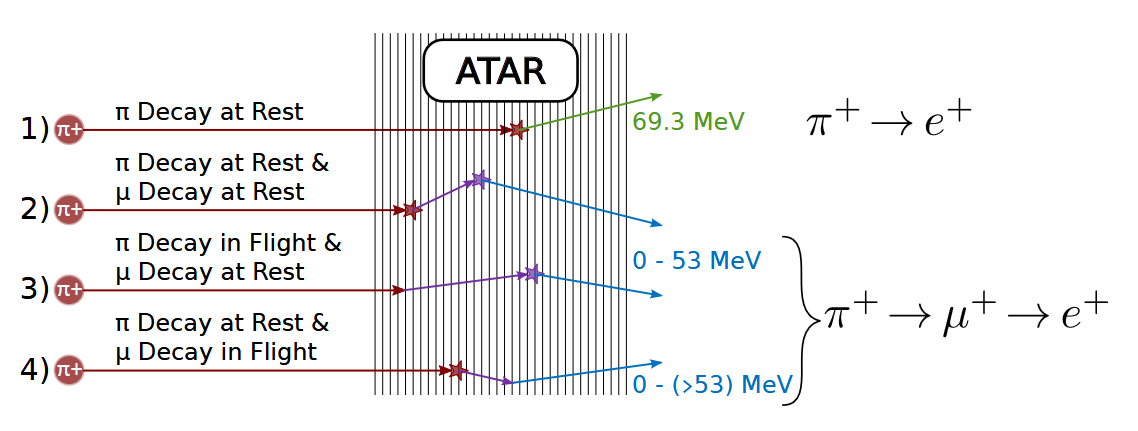
\includegraphics[width=0.86\textwidth]{../resources/figures/chapters/01_introduction/ATAR_decay_types}
  \caption{
    Schematic event topologies in the active target for the direct
    \(\pi\to e\nu\) signal channel, the dominant \(\pi\to\mu\to e\)
    normalization channel, and decay-in-flight backgrounds. The segmented ATAR
    distinguishes pion stops, muon stops, short muon tracks, prompt positrons,
    and delayed Michel positrons using spatial, timing, and energy-deposition
    information.
  }
  \label{fig:measurement-atar-decay-types}
\end{figure}

\FloatBarrier

PIONEER addresses these modes with an active target that provides four-
dimensional tracking and energy measurement. The design goal is position
resolution at the level of \(\withunit{150}{\micro\meter}\), timing below
\(\withunit{1}{\nano\second}\), and sensitivity to energy deposits ranging
from \(\order{\withunit{30}{\kilo\electronvolt}}\) positron signals to the
\(\order{\withunit{4000}{\kilo\electronvolt}}\) Bragg peaks of stopping pions
and muons. This information enables triggers and offline selections that
separate pion stops, muon stops, prompt positrons, delayed Michel positrons,
decays in flight, and pileup \cite{pioneer_proposal_2022,pioneer_rare_2022}.

The active target also plays a central role in characterizing the
low-energy \(\pi\to e\nu\) tail beneath the Michel spectrum. Information from
the target can identify and suppress ordinary \(\pi\to\mu\to e\) events
through observation of the intermediate \(\withunit{4.1}{\mega\electronvolt}\)
muon, tight timing cuts, particle-identification signatures, and reconstructed
decay topologies. In particular, tracking information and localized energy
deposition patterns help distinguish pion and muon decays in flight from true
direct pion decays. These selections allow the residual low-energy
\(\pi\to e\nu\) response tail to be measured and corrected for
\cite{pioneer_proposal_2022}.


\subsection{Beam and Rate Requirements}
\label{subsec:measurement-beam-rate}

The measurement requires a continuous-wave, low-momentum pion beam focused to
a small spot and tuned so that pions stop inside the active target. The
PIONEER Phase-I design is based on a beam momentum near
\(\withunit{55}{\mega\electronvolt\per c}\), with momentum bite of order
\(\pm\withunit{2}{\percent}\), and a stopped-pion rate near
\(\withunit{300}{\kilo\hertz}\). At this momentum, beamline separation can
strongly reduce incoming muon and positron backgrounds
\cite{pioneer_proposal_2022}.

The resulting event rate drives the need for fast triggering, waveform
digitization, and high-bandwidth data acquisition, but the experiment does not
attempt to record every pion stop as a full physics event. Instead, several
trigger classes select complementary event samples for detector monitoring,
signal enrichment, normalization, and background studies. The minimum-bias PI
trigger records an unbiased sample of stopped-pion events with a large
prescale. The CaloH trigger selects events with calorimeter energy above the
Michel endpoint, producing a sample strongly enriched in
\(\pi\to e\nu\) decays. The TRACK trigger records events with tracker activity
in a broad time window around the pion stop, providing a large normalization
sample dominated by ordinary \(\pi\to\mu\to e\) decays together with accidental
positrons from earlier stopped muons. Finally, the PROMPT trigger selects
early-time tracker activity shortly after the pion stop. This trigger is
particularly important for measuring the low-energy
\(\pi\to e\nu\) response tail beneath the Michel spectrum, which was a dominant
systematic uncertainty in previous \(R_{e/\mu}\) experiments. Additional
topology constraints from the active target can further suppress ordinary
\(\pi\to\mu\to e\) backgrounds in this prompt sample
\cite{kammel_pioneer_trigger,pioneer_proposal_2022}. For a stopped-pion rate near \(\withunit{300}{\kilo\hertz}\), these trigger
selections reduce the total physics-trigger rate to
\(\order{\withunit{10}{\kilo\hertz}}\), keeping event spacing, bandwidth, and
deadtime compatible with the DAQ design.

\begin{table}[htbp]
  \centering
  \caption{
    Representative trigger classes and approximate trigger rates for the
    PIONEER Phase-I \(R_{e/\mu}\) measurement, adapted from the PIONEER
    proposal \cite{pioneer_proposal_2022}. The trigger system separates
    unbiased pion samples, \(\pi\to e\nu\)-enhanced events, normalization
    samples, and prompt-tail studies while reducing the overall DAQ bandwidth.
  }
  \label{tab:pioneer-trigger-rates}
  \small
  \begin{tabular}{@{}lcccp{0.33\textwidth}@{}}
    \toprule
    Trigger & Prescale & Time Range (ns) & Rate (kHz) & Primary Purpose \\
    \midrule
    PI      & 1000 & $[-300,700]$ & 0.3 & Minimum-bias monitoring sample \\
    CaloH   & 1    & $[-300,700]$ & 0.1 & High-energy \(\pi\to e\nu\)-enhanced sample \\
    TRACK   & 50   & $[-300,700]$ & 3.4 & Normalization and accidental sample \\
    PROMPT  & 1    & $[2,32]$     & 5   & Prompt-tail and early-time studies \\
    \bottomrule
  \end{tabular}
\end{table}
